\section{Технический проект}
\subsection{Общая характеристика организации решения задачи}

Требуется спроектировать и разработать клиентскую(веб-сайт) и серверную часть программно-информационной системы.

Центральной задачей проекта является обеспечение пользователей доступом к библиотеке музыкальных треков и плейлистов через веб-интерфейс. 
В рамках проекта предусмотрена реализация технологий для поддержки непрерывного воспроизведения музыки  Разработка включает в себя создание бэкенд-системы, способной поддерживать стабильную работу сервиса.

\subsection{Обоснование выбора технологии проектирования}

Выбор технологии проектирования является ключевым аспектом в разработке любого программного продукта. Тщательный анализ возможных вариантов и сравнение их характеристик позволили определить оптимальное сочетание технологий, которые обеспечат выполнение всех функциональных требований и гарантируют удобство в дальнейшей поддержке и развитии проекта. 

\subsubsection{Описание используемых технологий и языков программирования}

В процессе разработки backend- и frontend-частей применяются различные технологии и языки программирования, обеспечивающие как простоту разработки, так и производительность конечной системы.

\subsubsection{Язык программирования Java}

Java — строго типизированный объектно-ориентированный язык программирования общего назначения, разработанный компанией Sun Microsystems (в последующем приобретённой компанией Oracle). Разработка ведётся сообществом, организованным через Java Community Process; язык и основные реализующие его технологии распространяются по лицензии GPL. Работает на принципе "<write once, run anywhere"> (WORA), что означает, что скомпилированный Java-код может запускаться на любой платформе без необходимости повторной компиляции. Это достигается за счёт Java Virtual Machine (JVM), которая интерпретирует байт-код Java для выполнения на любой операционной системе\cite{java}. 
В языке реализовано автоматическое управление памятью. Имеет бгатый набор стандартных коллекций: массив, список, стек и т.п.

\subsubsection{Фреймворк Spring}

Spring Framework - универсальный фреймворк для языка Java с открытым исходным кодом. Он предлагает набор модулей для решения типовых задач при разработке, таких как доступ к данным, аутентификация и авторизация, тестирование и другие. В центре фреймворка лежит контейнер инверсии управления, предоставляющий механизмы конфигурирования и управления Java объектами, что позволяет реализовать шаблон "<Внедерние зависимостей">\cite{springboot}.
Основные модули Spring:
\begin{itemize}
	\item Spring Boot - автоконфигурация проектов;
	\item Spring Data - управление данными приложения\cite{persist};
	\item Spring Security - конфигурация авторизации и аутентификации;
	\item Spring Cloud - средства для разработки приложений на основе микросервисной архитектуры\cite{springcloud}.
\end{itemize}

\subsubsection{Язык программирования JavaScript}

JavaScript является высокоуровневым, интерпретируемым языком программирования, который стал стандартом де-факто для веб-разработки на клиентской стороне\cite{js}. Изначально предназначенный для создания интерактивных элементов на веб-страницах, JavaScript со временем значительно расширил свои возможности и теперь используется в разнообразных сферах программирования. JavaScript поддерживает несколько парадигм программирования, что делает его исключительно гибким. 
JavaScript играет важную роль в разработке одностраничных приложений с помощью современных фреймворков и библиотек, таких как Angular, React и Vue.js, которые позволяют создавать интерактивные и масштабируемые пользовательские интерфейсы.

\subsubsection{Фреймворк Vue.js}

Vue.js — это прогрессивный JavaScript фреймворк, предназначенный для создания пользовательских интерфейсов. Основная его особенность заключается в постепенной адаптации: базовый уровень Vue.js фокусируется только на представлении (view layer), что делает его простым в интеграции с другими библиотеками или существующими проектами. Однако при необходимости Vue может легко функционировать и как часть полноценной экосистемы для разработки сложных одностраничных приложений (SPA)\cite{vue}. Фреймворк предоставляет готовые решения для маршрутизации (Vue Router), управления состоянием (Vuex и Pinia), что позволяет легко масштабировать приложение.

\subsection{Архитектура программной системы}

Разрабатываемый программный продукт реализован на основе клиент-серверной архитектуре\cite{arch2}. 
«Клиент — сервер» — это архитектура вычислительных или сетевых систем, где задачи или нагрузка распределяются между сервисами, предоставляемыми серверами, и клиентами, которые эти сервисы используют. Клиент и сервер представляют собой программное обеспечение, обычно расположенное на разных устройствах и взаимодействующее через сеть с использованием сетевых протоколов, хотя они могут находиться и на одном устройстве. Серверные программы ожидают запросы от клиентских программ и предоставляют им ресурсы, такие как данные (например, передача файлов через HTTP\cite{http}, FTP, потоковое мультимедиа или доступ к базам данных) или сервисные функции (например, работа с электронной почтой, обмен мгновенными сообщениями или просмотр веб-страниц).
Взаимодействие между клиентом и сервером реализовано на основе REST API\cite{springboot}\cite{webapi}. REST (от англ. REpresentational State Transfer — «передача репрезентативного состояния» или «передача „самоописываемого“ состояния») — это архитектурный стиль для взаимодействия компонентов распределенного приложения в сети. Проще говоря, REST определяет правила для организации кода серверного приложения, чтобы системы могли легко обмениваться данными и приложение было масштабируемым. REST представляет собой набор согласованных ограничений, учитываемых при проектировании распределенной гипермедиа-системы. В определенных случаях, таких как интернет-магазины и поисковые системы, использование REST приводит к повышению производительности и упрощению архитектуры. В общем смысле, компоненты в REST взаимодействуют аналогично взаимодействию клиентов и серверов во Всемирной паутине.

\subsubsection{Диаграмма компонентов}

Диаграмма компонентов отображает физическую структуру разрабатываемой системы, позволяя выявить архитектурные особенности путём установления взаимосвязей между программными компонентами. Эти компоненты могут представлять собой как исходный код, так и исполняемые файлы. Основные элементы этой диаграммы включают компоненты, интерфейсы и зависимости между ними, которые помогают в организации и понимании структуры системы. На рисунке \ref{frontendComponents:image} изображена диаграмма компонентов для клиентской части проектируемой системы\cite{uml}.

\begin{figure}[ht]
\center{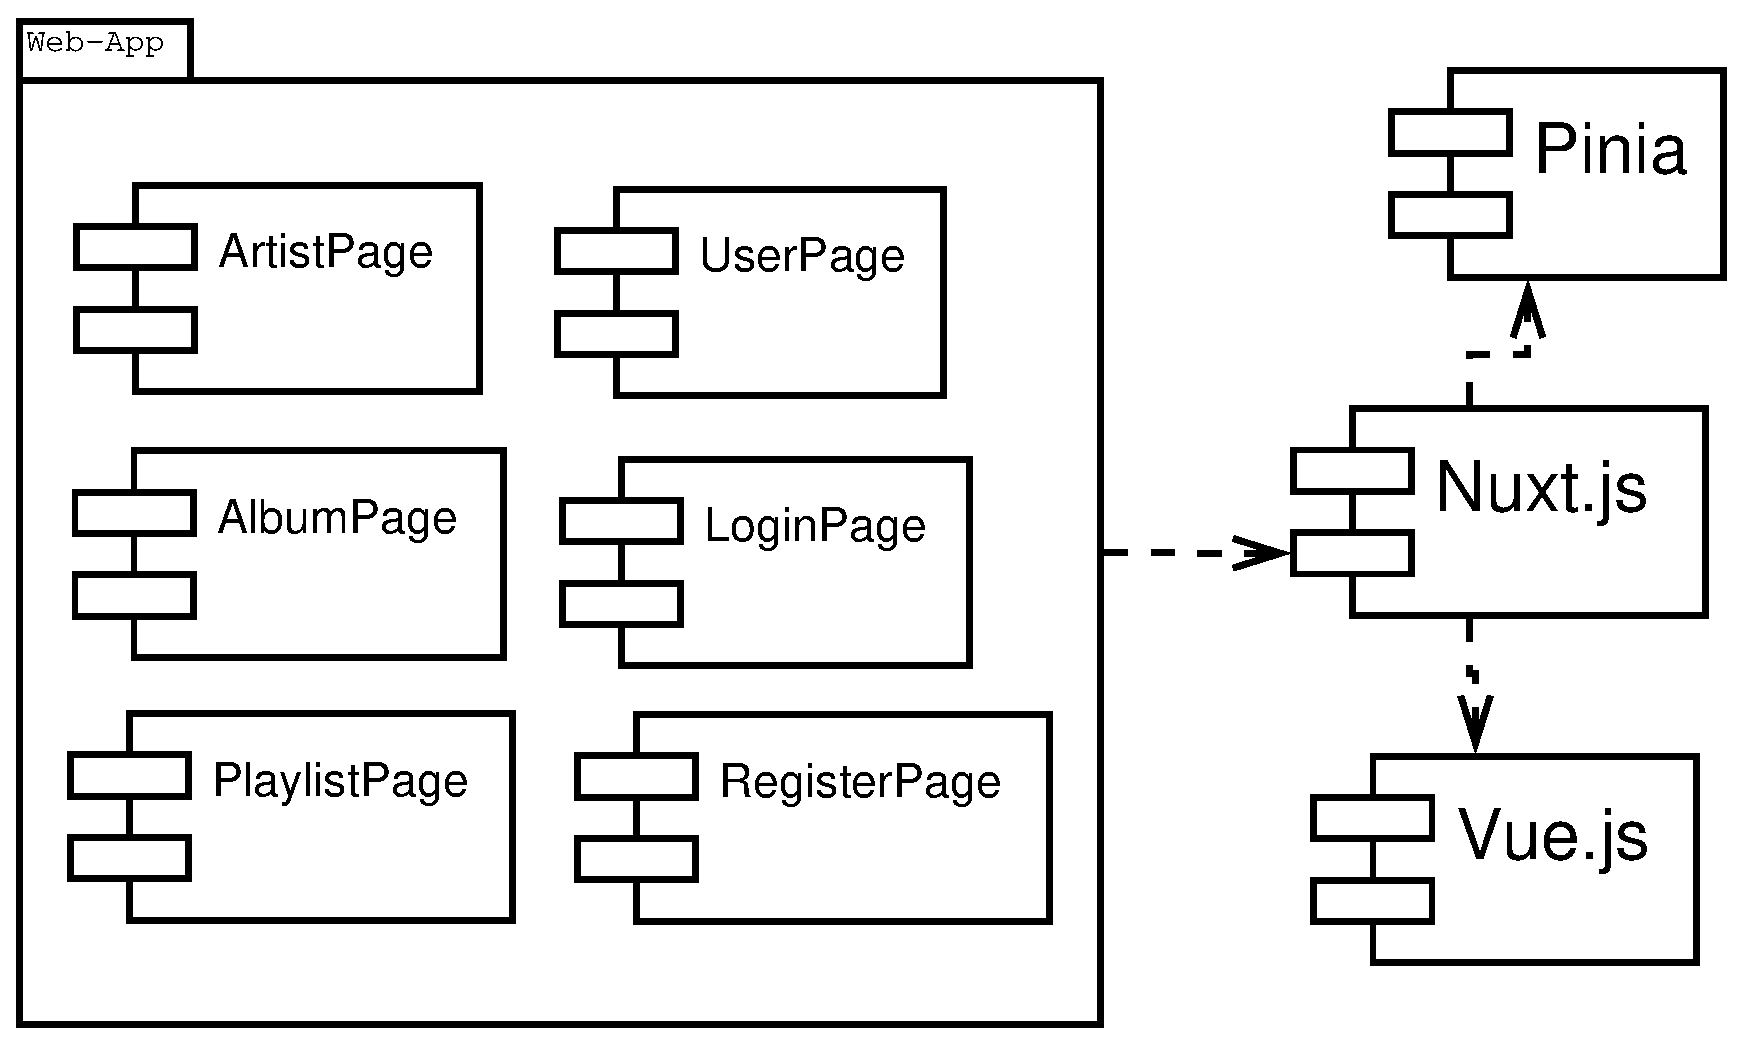
\includegraphics[width=1\linewidth]{frontendComponents}}
\caption{Диаграмма компонентов клиентской части}
\label{frontendComponents:image}
\end{figure}

На рисунке \ref{backendComp:image} изображена диаграмма компонентов для серверной части приложения.

\begin{figure}[ht]
	\center{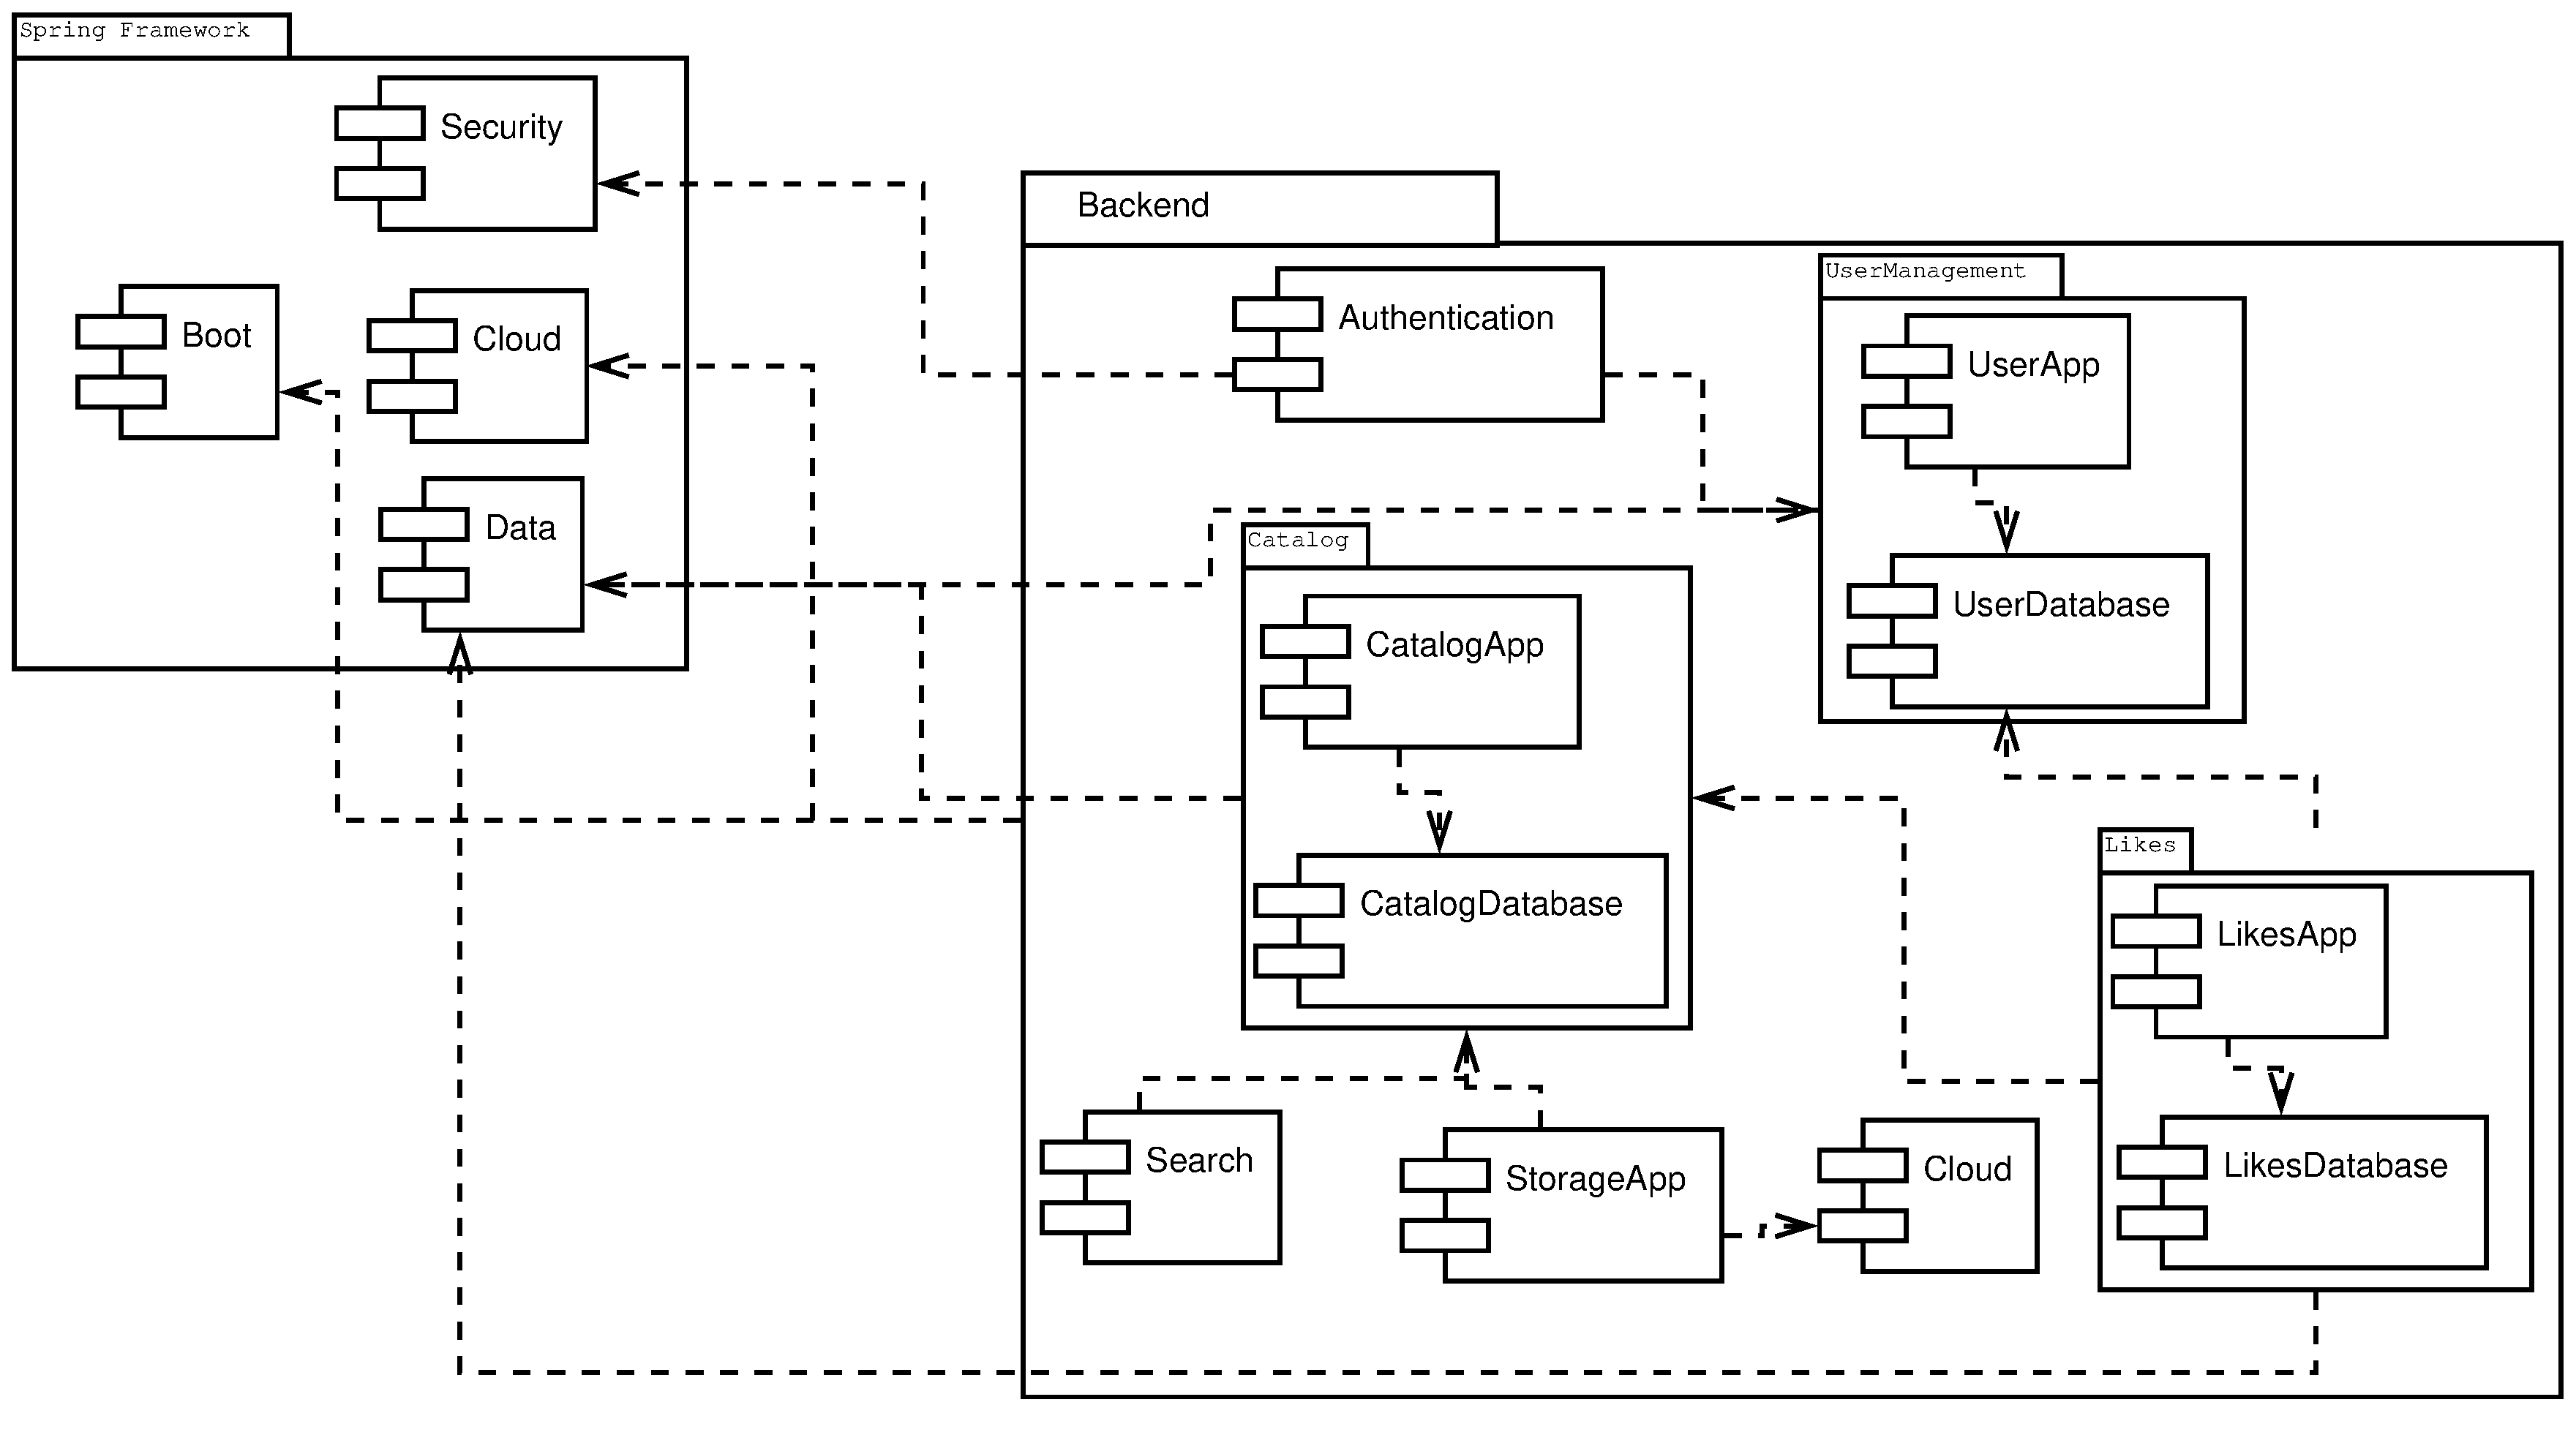
\includegraphics[width=1\linewidth]{backendComp}}
	\caption{Диаграмма компонентов клиентской части}
	\label{backendComp:image}
\end{figure}

Разрабатываемая программная система состоит из клиентской и серверной частей. Клиентская часть представляет собой одностраничное веб-приложение, доступное на любом устройстве, имеющем веб-браузер.
Серверная часть состоит из группы компонентов, отвечающих за разный функционал:
\begin{itemize}
	\item компонент аутентификации выполняет аутентификацию и авторизацию пользователей;
	\item компонент управления пользователями хранит данные пользователей, также отвечает за обработу запросов на изменение данных пользователей;
	\item компонент музыкального каталога отвечет за обрабатку запросов, связанные с музыкальным каталогом;
	\item компонент "<лайков"> хранит "<лайки"> пользователей, обрабатывает запросы на установку и удаление "<лайков">;
	\item компонент поиска обрабатывает поисковые запросы пользователей по музыкальному каталогу;
	\item фйловое хранилище хранит аудиофайлы, обложки альбомов и плейлистов, фото пользоватей.
\end{itemize}

\subsubsection{Компоненты клиентской части}

Клиентская часть представлена приложением на Nuxt3. Страницы Nuxt3 представляют собой Single File Component (однофайловые компоненты) Vue.js, которые совмещают в одном файле шаблон HTML-разметки, стили CSS и логику управления состоянием и данными, написанную на TypeScript.
Разработаны следующие страницы:
\begin{itemize}[]
	\item LoginPage - страница авторизации;
	\item RegisterPage - страница регистрации;
	\item HomePage - страница авторизации;
	\item SearchResultPage - страница авторизации;
	\item ArtistPage - страница исполнителя;
	\item AlbumPage - страница альбома;
	\item PlaylistPage - страница плейлиста;
	\item UserPage - страница пользователя.
\end{itemize}

\subsubsection{Абстракция данных программной системы}
На рисунке \ref{domainClass:image} представлена диаграмма классов предметной области данной системы.

\begin{figure}[ht]
	\center{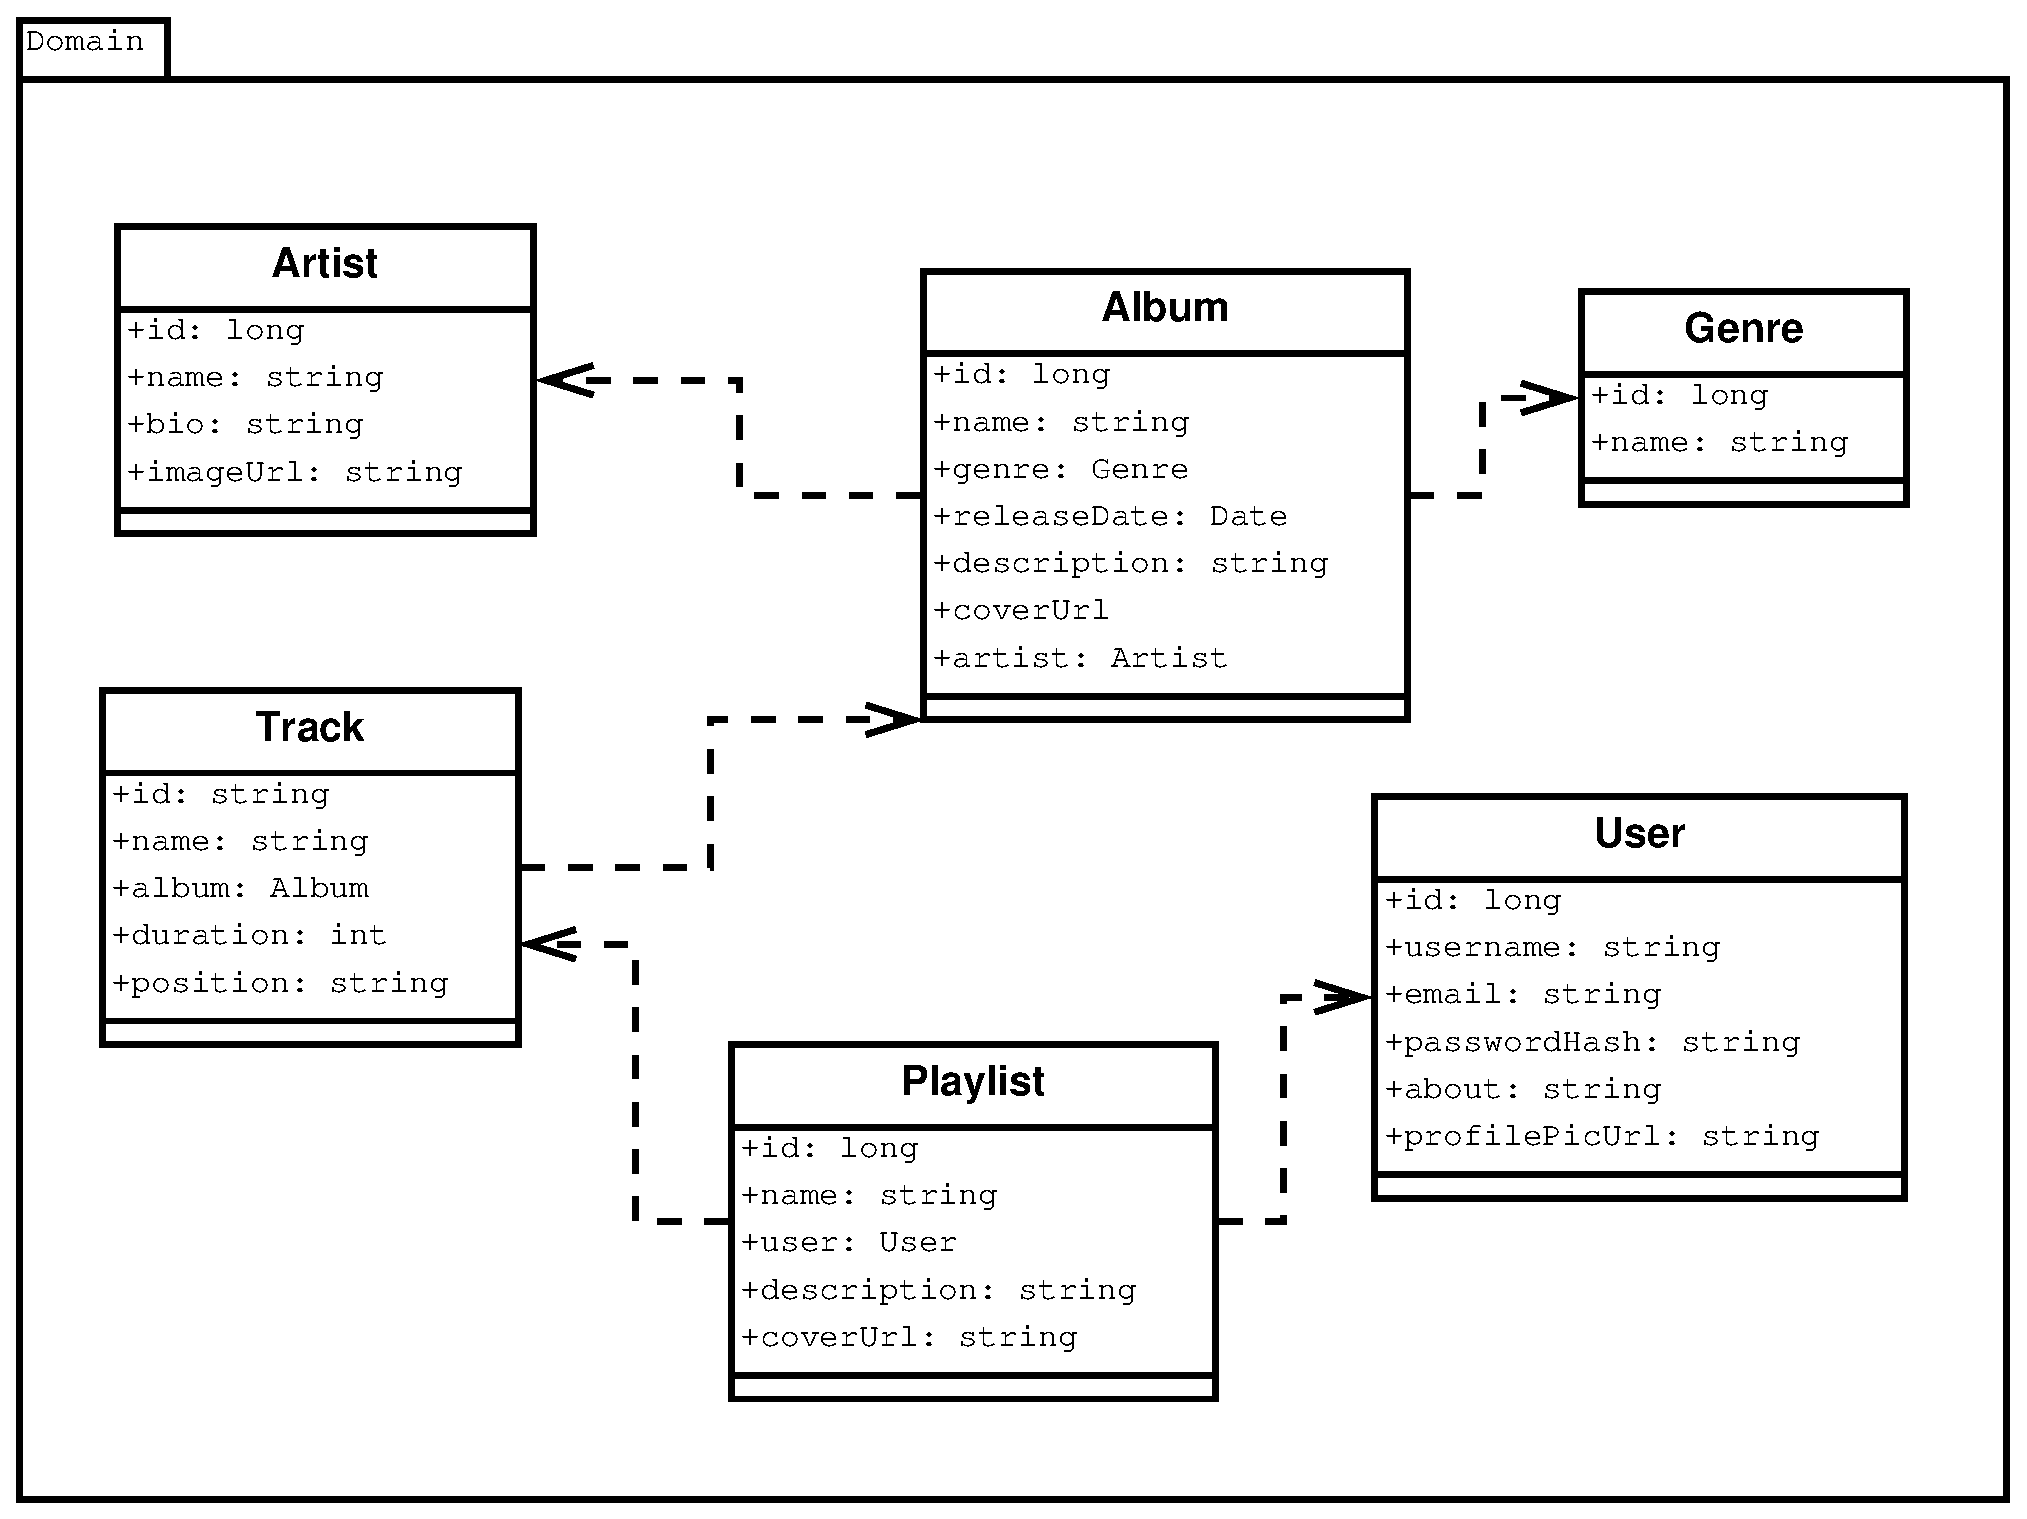
\includegraphics[width=1\linewidth]{domainClass}}
	\caption{Карта маршрутов}
	\label{domainClass:image}
\end{figure}

\subsubsection{Конечные точки серверной части}

Для организации взаимодействия клиентской части с бизнес-логикой приложения были определены конечные точки. На рисунке \ref{routeMap:image} представлена карта маршрутов, представляющая схематическое изображение конечных точек.

\begin{figure}[ht]
	\center{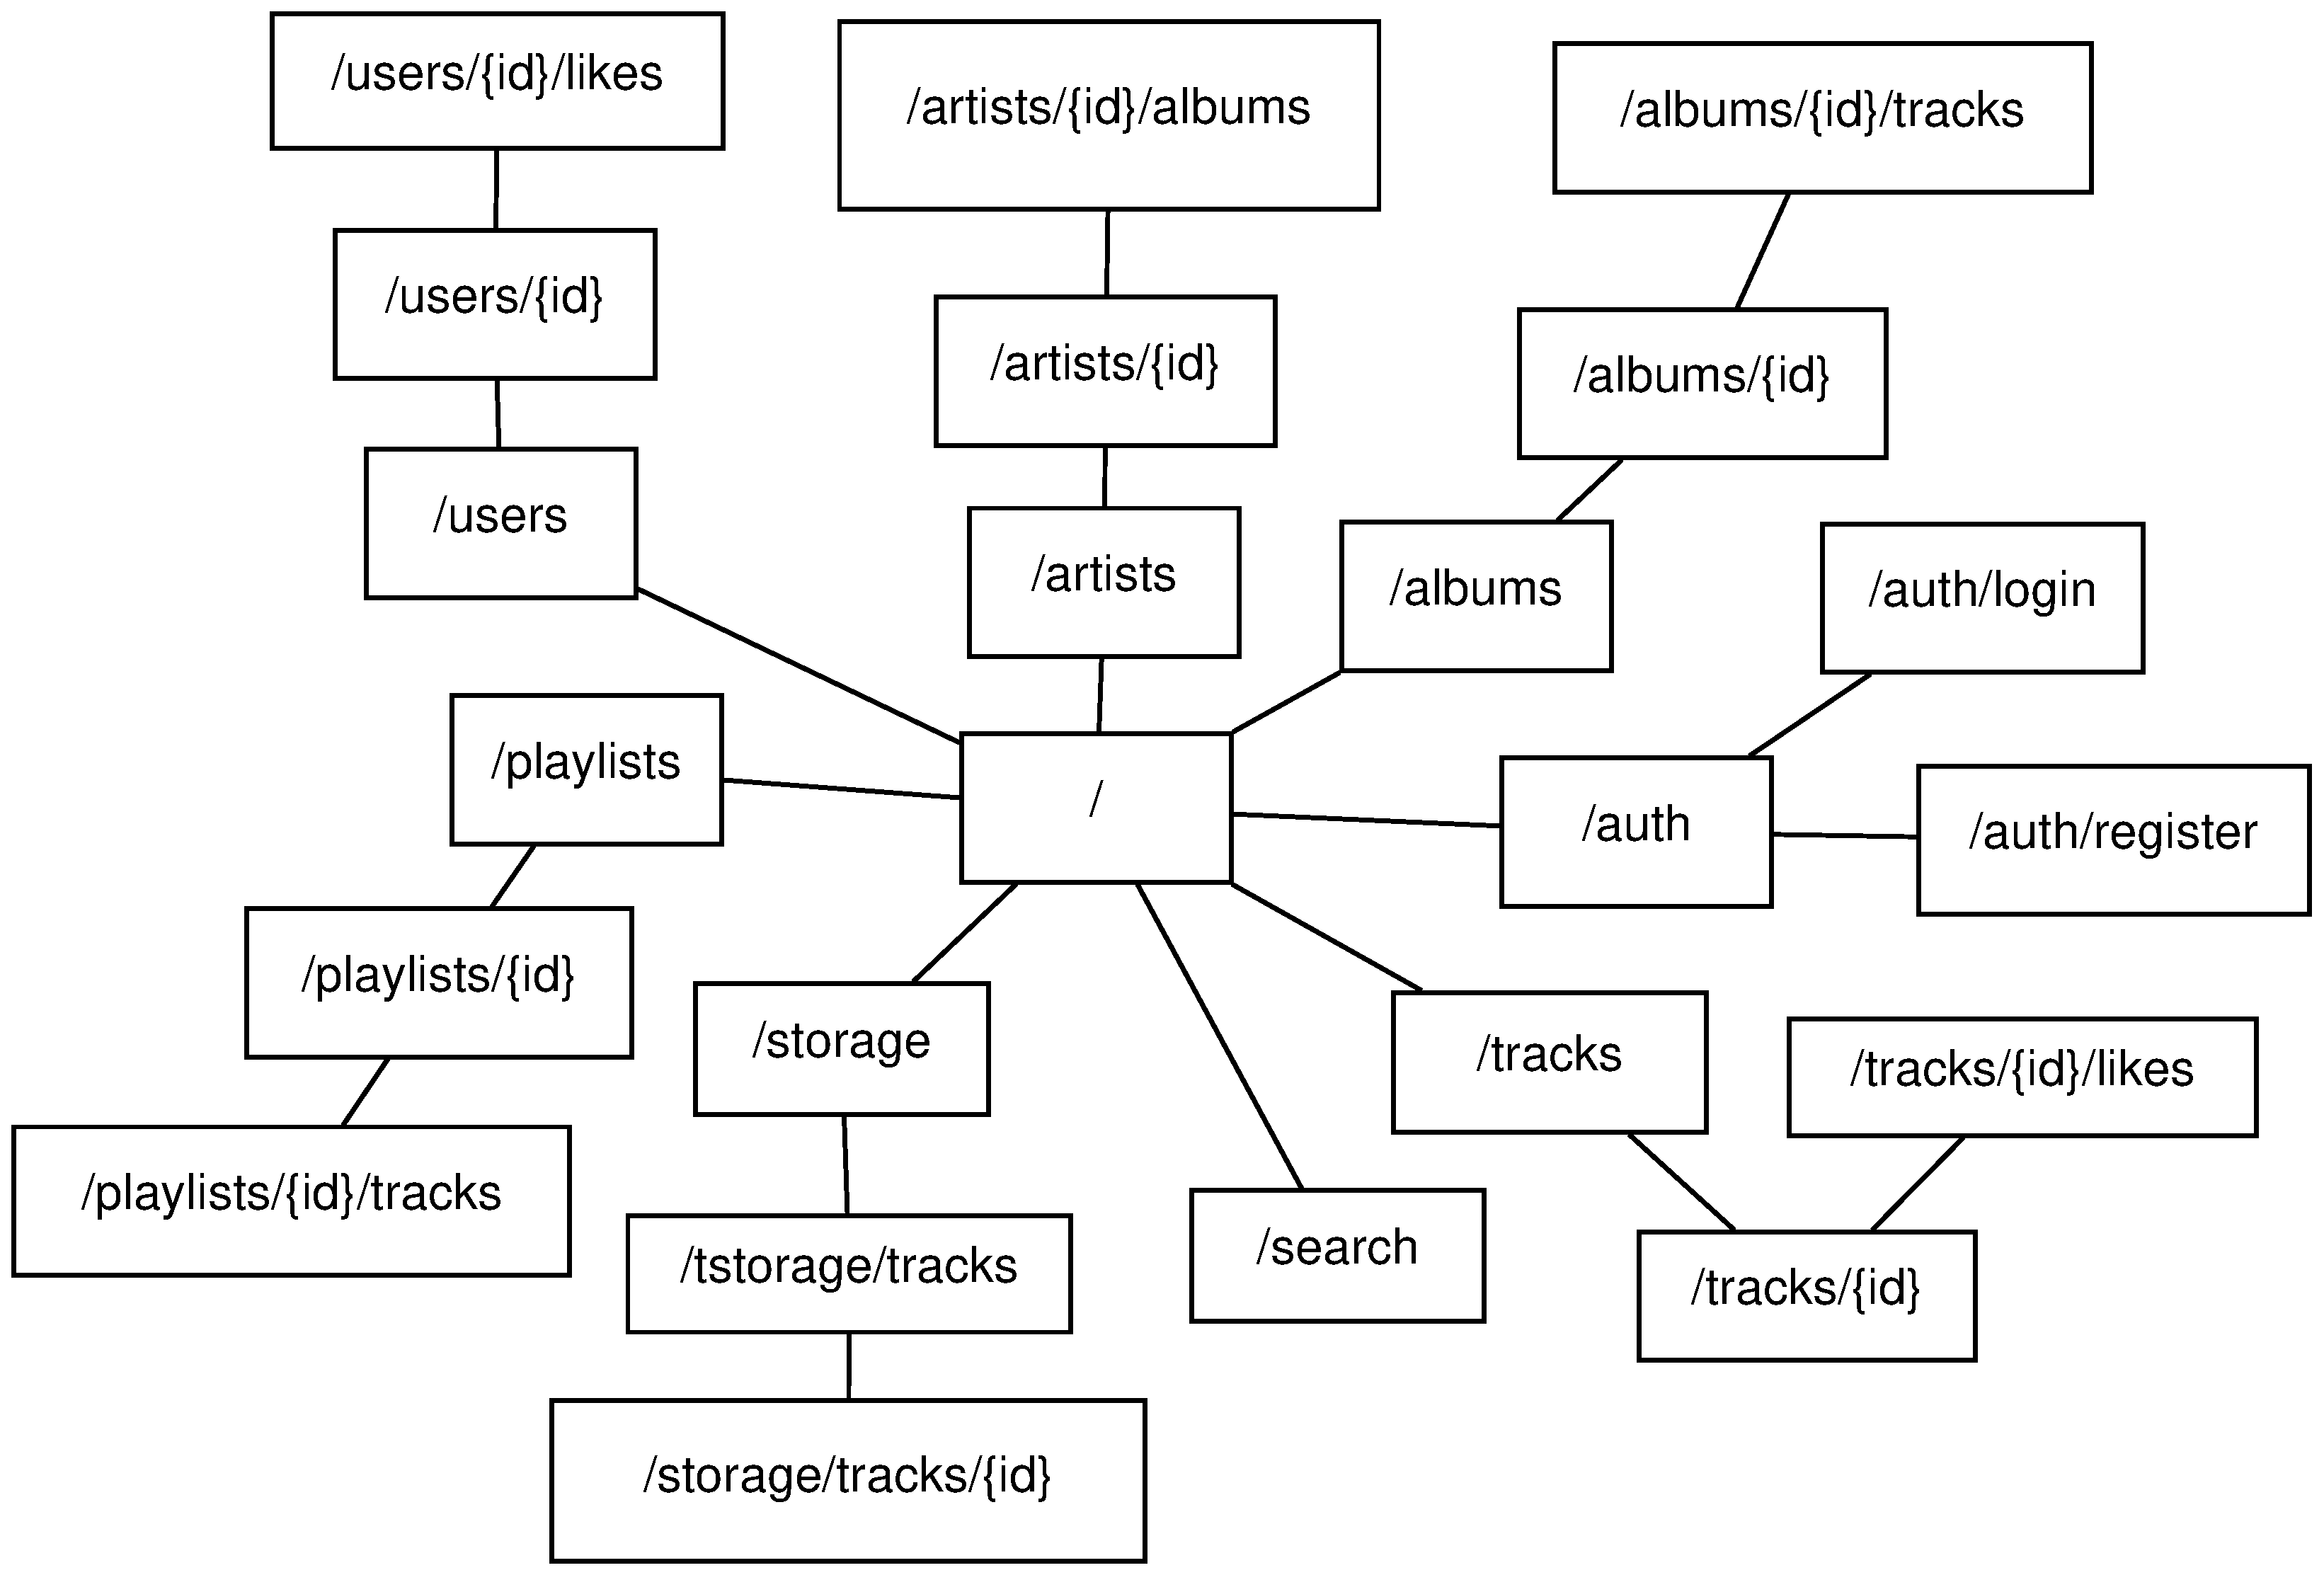
\includegraphics[width=1\linewidth]{routeMap}}
	\caption{Карта маршрутов}
	\label{routeMap:image}
\end{figure}

GET /artists/{id} - предназначен для получения данных об артисте. Принимает параметр id, описывающий идентификатор артиста.

GET /artists/{id}/albums - предназначен для получения списка альбомов артиста. Принимает параметр id, описывающий идентификатор артиста.

GET /albums/{id} - предназначен для получения данных об альбоме. Принимает параметр id, описывающий идентификатор альбома.

GET /albums/{id}/tracks - предназначен для получения списка треков альбома. Принимает параметр id, описывающий идентификатор альбома.

GET /playlists/{id} - предназначен для получения данных о плейлисте. Принимает параметр id, описивающий идентификатор плейлиста.

GET /playlists/{id}/tracks - предназначен для получения списка треков в плейлисте. Принимает параметр id, описивающий идентификатор плейлиста.

POST /playlists - предназначен для создания плейлиста. Принимает в теле запроса JSON-объект, описывающий создаваемый плейлист.

DELETE /playlists/{id} - предназначен для удаления плейлиста. Принимает параметр id, описивающий идентификатор плейлиста.

DELETE /playlists/{id}/tracks - предназначен для удаления треков из плейлиста. Принимает в теле запроса JSON-объект, описывающий список идентификаторов треков, удаляемых из плейлиста и параметр id, описывающий идентификатор плейлиста, из которого удаляются треки. 

PUT /playlists/{id} - предназначен для изменения данных (названия, описания) плейлиста. Принимает в теле запроса JSON-объект, описывающий новые данные о плейлисте. В качестве параметра пути принимает id, описывающий идентификатор плейлиста.

POST /playlists/{id}/tracks - предназначен для добавления треков в плейлист. Принимает в теле запроса JSON-объект, описывающий список идентификаторов треков, добавляемых в плейлист и параметр id, описывающий идентификатор плейлиста, в который добавляются треки. 

POST /auth/login - предназначен для входа пользователя в приожение. Принимает в теле запроса JSON-объект, описывающий данные для аутентификации.

POST /auth/register - предназначен для регистрации пользователя в приложении.  Принимает в теле запроса JSON-объект, описывающий данные для регистрации.

GET /users/{id} - предназначен для получения информации о пользователе. Принимает параметр id, описывающий идентификатор пользователя.

GET /users/likes - предназначен для получения "<лайков"> пользователя.

GET /track/{id}/likes - предназначен для получения "<лайков"> трека. Принимает параметр id, описывающий идентификатор трека, "<лайки"> которого необходимо получить.

POST /track/{id}/likes - предназначен для установки "лайка" трека. Принимает параметр id, описывающий идентификатор трека, "<лайк"> которому необходимо поставить.

POST /track/{id}/likes - предназначен для установки "<лайка"> трека. Принимает параметр id, описывающий идентификатор трека, "<лайк"> которому необходимо поставить.

DELETE /track/{id}/likes - предназначен для удаления "<лайка"> трека. Принимает параметр id, описывающий идентификатор трека, с которого необходимо убрать "<лайк">.

GET /storage/tracks/{id} - предназначен для получения аудиопотока. Принимает параметр id, описывающий идентификатор трека.

GET /search?query={query}\&type={}type - предназначен для поиска в музыкальном каталоге. Принимает строковый параметр query, являющийся строкой запроса, и численный параметр type, обозначающий, в какой категории производится поиск.


\subsection{Проект данных программной системы}

Исходя из требований технического задания, программноинформационная система должна взаимодействовать с двумя типами баз
данных.
SQL\cite{sql1} (реляционные) и NoSQL (нереляционные) являются разными подходами к работе с данными и их хранением. Реляционные базы данных представляют собой базы данных, которые используются для хранения и предоставления доступа к взаимосвязанным элементам информации. Реляционные базы данных основаны на реляционной модели — табличном способе представления данных. Каждая строка, содержащая в таблице такой базы данных, представляет собой запись с уникальным идентификатором, который называют ключом. Столбцы таблицы имеют атрибуты данных, а каждая запись обычно содержит значение для каждого атрибута, что дает возможность легко устанавливать взаимосвязь между элементами данных. Реляционная модель наиболее эффективно поддерживает целостность данных во всех приложениях и копиях (экземплярах) базы данных благодаря соответствию принципам ACID, подразумевающих под собой:
\begin{itemize}
	\item атомарность (англ. atomicity) - никакая транзакция не будет зафиксирована в системе частично;
	\item согласованность (англ. consistency) - каждая успешная транзакция по определению фиксирует только допустимые результаты;
	\item изолированность (англ. isolation) - во время выполнения транзакции параллельные транзакции не должны оказывать влияния на её результат;
	\item устойчивость (англ. durability) - независимо от проблем на нижних уровнях изменения, сделанные успешно завершённой транзакцией, должны остаться сохранёнными после возвращения системы в работу.
\end{itemize}
В отличие от реляционных систем, нереляционные базы данных предлагают гибкость схем данных и способны эффективно масштабироваться для обработки больших объемов данных. NoSQL базы данных часто используют различные структуры данных, такие как ключ-значение, документы, графы и широкие столбцы, что позволяет оптимизировать производительность и удобство разработки в зависимости от характера данных и запросов. Эти системы обычно обеспечивают высокую производительность операций чтения и записи и хорошо подходят для приложений с большими объемами неструктурированных данных. При этом они не обеспечивают такой же устойчивости данных, как реляционный базы.
Основное отличие между SQL и NoSQL заключается в подходах к консистентности данных, масштабируемости и гибкости управления схемами. Реляционные базы данных предпочтительны, когда необходима высокая степень согласованности и точности данных, в то время как нереляционные системы лучше подходят для случаев, когда приоритетны горизонтальное масштабирование и гибкость структуры данных. 

\subsubsection{Описание сущностей серверной части}

В таблице \ref{artist:table} приведены атрибуты и их описание для сущности "<Артист">.

\renewcommand{\arraystretch}{0.8} 
\begin{xltabular}{\textwidth}{|l|l|p{1.7cm}|X|}
	\caption{Атрибуты сущности "<Артист">\label{artist:table}}\\ \hline
	\centrow Поле & \centrow Тип & \centrow Обяза\-тельное & \centrow Описание \\ \hline
	\thead{1} & \thead{2} & \centrow 3 & \centrow 4 \\ \hline
	\endfirsthead
	\continuecaption{Продолжение таблицы \ref{artist:table}}
	\thead{1} & \thead{2} & \centrow 3 & \centrow 4 \\ \hline
	\finishhead
	artist\_id & integer & да & Уникальный идентификатор, автогенерируемый \\ \hline 
	name & character varying(128) & да & Имя артиста \\ \hline 
	bio & character varying(256) & нет & Краткая биорафия \\ \hline 
	image\_url & character varying(256) & нет & Фото артиста \\ \hline 
\end{xltabular}
\renewcommand{\arraystretch}{1.0} 

В таблице \ref{album:table} приведены атрибуты и их описание для сущности "<Альбом">.

\renewcommand{\arraystretch}{0.8} 
\begin{xltabular}{\textwidth}{|l|l|p{1.7cm}|X|}
	\caption{Атрибуты сущности "<Альбом">\label{album:table}}\\ \hline
	\centrow Поле & \centrow Тип & \centrow Обяза\-тельное & \centrow Описание \\ \hline
		\thead{1} & \thead{2} & \centrow 3 & \centrow 4 \\ \hline
	\endfirsthead
	\continuecaption{Продолжение таблицы \ref{album:table}}
	\thead{1} & \thead{2} & \centrow 3 & \centrow 4 \\ \hline
	\finishhead
	album\_id & integer & да & Уникальный идентификатор альбома, автогенерируемый \\ \hline
	artist\_id & integer & да & Идентификатор артиста, внешний ключ \\ \hline
	name & character varying(128) & да & Название альбома \\ \hline
	release\_date & date & да & Дата выпуска \\ \hline
	type & album\_type & да & Тип альбома \\ \hline
	cover\_url & character varying(256) & да & URL обложки альбома \\ \hline
	genre\_id & integer & да & Идентификатор жанра, внешний ключ \\ \hline
\end{xltabular}
\renewcommand{\arraystretch}{1.0}
В таблице \ref{track:table} приведены атрибуты и их описание для сущности "<Трек">.
\renewcommand{\arraystretch}{0.8} 
\begin{xltabular}{\textwidth}{|l|l|p{1.7cm}|X|}
	\caption{Атрибуты сущности "<Трек">\label{track:table}}\\ \hline
	\centrow Поле & \centrow Тип & \centrow Обяза\-тельное & \centrow Описание \\ \hline
		\thead{1} & \thead{2} & \centrow 3 & \centrow 4 \\ \hline
	\endfirsthead
	\continuecaption{Продолжение таблицы \ref{track:table}}
	\thead{1} & \thead{2} & \centrow 3 & \centrow 4 \\ \hline
	\finishhead
	track\_id & integer & да & Уникальный идентификатор трека, автогенерируемый \\ \hline
	album\_id & integer & да & Идентификатор альбома, внешний ключ \\ \hline
	name & character varying(128) & да & Название трека \\ \hline
	duration & integer & да & Длительность трека в секундах \\ \hline
	position & integer & да & Позиция трека в альбоме \\ \hline
\end{xltabular}
\renewcommand{\arraystretch}{1.0}
В таблице \ref{playlist:table} приведены атрибуты и их описание для сущности "<Плейлист">.
\renewcommand{\arraystretch}{0.8} 
\begin{xltabular}{\textwidth}{|l|l|p{1.7cm}|X|}
	\caption{Атрибуты сущности "<Плейлист">\label{playlist:table}}\\ \hline
	\centrow Поле & \centrow Тип & \centrow Обяза\-тельное & \centrow Описание \\ \hline
		\thead{1} & \thead{2} & \centrow 3 & \centrow 4 \\ \hline
	\endfirsthead
	\continuecaption{Продолжение таблицы \ref{playlist:table}}
	\thead{1} & \thead{2} & \centrow 3 & \centrow 4 \\ \hline
	\finishhead
	playlist\_id & integer & да & Уникальный идентификатор плейлиста, автогенерируемый \\ \hline
	user\_login & character varying(128) & да & Логин пользователя, создавшего плейлист \\ \hline
	name & character varying(128) & да & Название плейлиста \\ \hline
	cover\_url & character varying(256) & нет & URL обложки плейлиста \\ \hline
\end{xltabular}
\renewcommand{\arraystretch}{1.0}
В таблице \ref{playlisttrack:table} приведены атрибуты и их описание для сущности "<Связь плейлист-трек">.
\renewcommand{\arraystretch}{0.8} 
\begin{xltabular}{\textwidth}{|l|l|p{1.7cm}|X|}
	\caption{Атрибуты сущности "<Связь плейлист-трек>"\label{playlisttrack:table}}\\ \hline
	\centrow Поле & \centrow Тип & \centrow Обяза\-тельное & \centrow Описание \\ \hline
		\thead{1} & \thead{2} & \centrow 3 & \centrow 4 \\ \hline
	\endfirsthead
	\continuecaption{Продолжение таблицы \ref{playlisttrack:table}}
	\thead{1} & \thead{2} & \centrow 3 & \centrow 4 \\ \hline
	\finishhead
	playlist\_playlist\_id & integer & да & Идентификатор плейлиста, внешний ключ \\ \hline
	track\_track\_id & integer & да & Идентификатор трека, внешний ключ \\ \hline
\end{xltabular}
\renewcommand{\arraystretch}{1.0}
В таблице \ref{genre:table} приведены атрибуты и их описание для сущности "<Жанр">.
\renewcommand{\arraystretch}{0.8} 
\begin{xltabular}{\textwidth}{|l|l|p{1.7cm}|X|}
	\caption{Атрибуты сущности "<Жанр">\label{genre:table}}\\ \hline
	\centrow Поле & \centrow Тип & \centrow Обяза\-тельное & \centrow Описание \\ \hline
		\thead{1} & \thead{2} & \centrow 3 & \centrow 4 \\ \hline
	\endfirsthead
	\continuecaption{Продолжение таблицы \ref{genre:table}}
	\thead{1} & \thead{2} & \centrow 3 & \centrow 4 \\ \hline
	\finishhead
	genre\_id & integer & да & Уникальный идентификатор жанра, автогенерируемый \\ \hline
	name & character varying & да & Название жанра \\ \hline
\end{xltabular}
\renewcommand{\arraystretch}{1.0}
В таблице \ref{user:table} приведены атрибуты и их описание для сущности "<Пользователь">.
\renewcommand{\arraystretch}{0.8} 
\begin{xltabular}{\textwidth}{|l|l|p{1.7cm}|X|}
	\caption{Атрибуты сущности "<Пользователь">\label{user:table}}\\ \hline
	\centrow Поле & \centrow Тип & \centrow Обяза\-тельное & \centrow Описание \\ \hline
		\thead{1} & \thead{2} & \centrow 3 & \centrow 4 \\ \hline
	\endfirsthead
	\continuecaption{Продолжение таблицы \ref{user:table}}
	\thead{1} & \thead{2} & \centrow 3 & \centrow 4 \\ \hline
	\finishhead
	user\_id & integer & да & Уникальный идентификатор пользователя, автогенерируемый \\ \hline 
	username & character varying(128) & да & Имя пользователя, уникальное в системе \\ \hline 
	email & character varying(256) & да & Электронная почта пользователя, уникальная в системе \\ \hline 
	password\_hash & character varying(256) & да & Хеш пароля для безопасности аутентификации \\ \hline 
	password\_salt & character varying(256) & да & Соль для хеширования пароля, уникальная для каждого пользователя \\ \hline 
	bio & text & нет & Краткая биография пользователя, необязательное поле \\ \hline 
	photo & character varying(256) & нет & URL фотографии профиля пользователя \\ \hline 
\end{xltabular}
\renewcommand{\arraystretch}{1.0}
В таблице \ref{like:table} приведены атрибуты и их описание для сущности "<Лайк">.
\renewcommand{\arraystretch}{0.8} 
\begin{xltabular}{\textwidth}{|l|l|p{1.7cm}|X|}
	\caption{Атрибуты сущности "<Лайк">\label{like:table}}\\ \hline
	\centrow Поле & \centrow Тип & \centrow Обяза\-тельное & \centrow Описание \\ \hline
		\thead{1} & \thead{2} & \centrow 3 & \centrow 4 \\ \hline
	\endfirsthead
	\continuecaption{Продолжение таблицы \ref{like:table}}
	\thead{1} & \thead{2} & \centrow 3 & \centrow 4 \\ \hline
	\finishhead
	\_id & ObjectId & да & Уникальный идентификатор лайка, автогенерируемый \\ \hline 
	user\_id & Long & да & Идентификатор пользователя, который поставил лайк \\ \hline 
	track\_id & Long & да & Идентификатор трека, которому поставлен лайк \\ \hline 
\end{xltabular}
\renewcommand{\arraystretch}{1.0}
\subsection{Проектирование пользовательского интерфейса}

После анализа требований к интерфейсу пользователя\cite{ui}, описанных в разделе технического задания, был разработан графический интерфейс для взаимодействия с приложением. Интерфейс разработан с применением javaScript- фреймворка Nuxt.js, основанного на Vue.js. Для стилизации элементов был использован CSS 3.
На представленных ниже рисунках числами обозначены элементы графического интерфейса.
На рисунке \ref{regMaket:image} представлен макет страницы регистрации. Элементы страницы регистрации:
\begin{enumerate}
	\item Форма регистрации.
	\item Поле ввода имени пользователя.
	\item Поле ввода электронной почты.
	\item Поле ввода пароля.
	\item Поле подтверждения пароля.
	\item Кнопка подтверждения формы.
\end{enumerate} 

\begin{figure}[ht]
	\center{\includegraphics[width=1\linewidth]{regMaket}}
	\caption{Макет страницы регистрации}
	\label{regMaket:image}
\end{figure}
На рисунке \ref{loginMaket:image} представлен макет страницы входа. Элементы страницы входа:
\begin{enumerate}
	\item Форма входа.
	\item Поле ввода электронной почты.
	\item Поле ввода пароля.
	\item Кнопка подтверждения формы.
	\item Ссылка на страницу регистрации.
\end{enumerate} 
\begin{figure}[ht]
	\center{\includegraphics[width=0.95\linewidth]{loginMaket}}
	\caption{Макет страницы входа}
	\label{loginMaket:image}
\end{figure}
На рисунке \ref{artistMaket:image} представлен макет страницы исполнителя. Элементы страницы исполнителя:
\begin{samepage}
	\begin{enumerate}
		\item Фото исполнителя.
		\item Информация о исполнителе.
		\item Список альбомов исполнителя.
		\item Карточка с информацией об альбоме.
		\item Ссылка на страницу альбома.
	\end{enumerate} 
\end{samepage}
\begin{figure}[ht]
	\center{\includegraphics[width=0.8\linewidth]{artistMaket}}
	\caption{Макет страницы исполнителя}
	\label{artistMaket:image}
\end{figure}
На рисунке \ref{albumMaket:image} представлен макет страницы альбома. Элементы страницы альбома:
\begin{enumerate}
	\item Обложка альбома.
	\item Информация об альбоме.
	\item Список треков.
	\item Строка трека.
	\item Информация о треке.
	\item Кнопка запуска проигрывания.
\end{enumerate} 
\begin{figure}[ht]
	\center{\includegraphics[width=0.85\linewidth]{albumMaket}}
	\caption{Макет страницы альбома}
	\label{albumMaket:image}
\end{figure}

